
\begin{frame}
	\vspace{2cm}
	\begin{center}
		{\Huge\textbf{\textcolor{copenhagenred}{Parallel Tempering MCMC}}}
		\vspace{1cm}

		\rule{4cm}{3pt}
		\vspace{2cm}
	\end{center}
\end{frame}

\begin{frame}{The Problem and Solution}
	\begin{columns}
		\column{0.48\textwidth}
		\textbf{The Problem:}
		\begin{itemize}
			\item Standard MCMC gets stuck in local modes
			\item Can't explore separated peaks
			\item Dilemma: small steps (stuck) vs. large steps (rejected)
		\end{itemize}

		\textbf{The Solution: Temperature Ladder}
		\begin{itemize}
			\item Run $N$ chains targeting $\pi^{\gamma_n}$
			\item $0 < \gamma_1 < \cdots < \gamma_N = 1$
			\item \textcolor{red}{Hot ($\gamma \approx 0$)}: Explores freely
			\item \textcolor{blue}{Cold ($\gamma = 1$)}: Exploits peaks
		\end{itemize}

		\column{0.48\textwidth}
		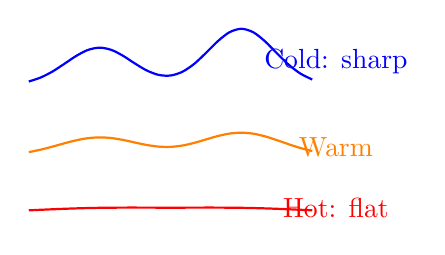
\begin{tikzpicture}[scale=0.6]
			% Hot chain
			\draw[red,thick] plot[smooth,domain=-3:3] (\x,{0.3 + 0.1*exp(-(\x+1.5)^2/4) + 0.1*exp(-(\x-1.5)^2/4)});
			\node[red] at (3.5,0.4) {Hot: flat};

			% Medium chain  
			\draw[orange,thick] plot[smooth,domain=-3:3] (\x,{1.5 + 0.4*exp(-(\x+1.5)^2/1.5) + 0.5*exp(-(\x-1.5)^2/1.5)});
			\node[orange] at (3.5,1.7) {Warm};

			% Cold chain
			\draw[blue,thick] plot[smooth,domain=-3:3] (\x,{3 + 0.8*exp(-(\x+1.5)^2) + 1.2*exp(-(\x-1.5)^2)});
			\node[blue] at (3.5,3.5) {Cold: sharp};

		\end{tikzpicture}
	\end{columns}

	\vspace{0.2cm}
	\textbf{Key Insight}
	Different temperatures see the same distribution differently - hot chains explore, cold chains exploit
\end{frame}

\begin{frame}{The Temperature Mechanism}
	\begin{block}{Key Idea: Tempered Distributions}
		Define a family of distributions indexed by inverse temperature $0 < \gamma_1 < \gamma_2 < \ldots < \gamma_N = 1$:
		$$\pi_{\gamma_n}(x) \propto \pi(x)^{\gamma_n}$$
		where $n=1, \ldots, N$ and $\pi(x)$ is our target distribution.
	\end{block}

	\begin{columns}
		\column{0.5\textwidth}
		\textbf{Properties:}
		\begin{itemize}
			\item $\gamma_N = 1$: Original target distribution
			\item $\gamma_1 \approx 0$: Uniform, explores broadly
		\end{itemize}

		\column{0.5\textwidth}
		\begin{tikzpicture}[scale=0.7]
			\begin{axis}[
					xlabel={$x$},
					ylabel={$\pi_{\gamma}(x)$},
					ymin=0, ymax=1,
					xmin=-4, xmax=4,
					height=5cm,
					width=7cm,
					legend pos=north east,
					cycle list name=color list
				]
				% Different inverse temperatures (gamma values)
				\addplot[copenhagenred, thick, samples=100, domain=-4:4]
				{0.3*exp(-2*(x+2)^2) + 0.7*exp(-2*(x-1.5)^2)};
				\addlegendentry{$\gamma=1$}

				\addplot[copenhagenred!70, thick, dashed, samples=100, domain=-4:4]
				{(0.3*exp(-2*(x+2)^2) + 0.7*exp(-2*(x-1.5)^2))^(1/2)};
				\addlegendentry{$\gamma=0.5$}

				\addplot[copenhagenred!40, thick, dotted, samples=100, domain=-4:4]
				{(0.3*exp(-2*(x+2)^2) + 0.7*exp(-2*(x-1.5)^2))^(1/4)};
				\addlegendentry{$\gamma=0.25$}
			\end{axis}
		\end{tikzpicture}
	\end{columns}
\end{frame}

\begin{frame}{Parallel Chains Architecture}
	\begin{center}
		\begin{tikzpicture}[scale=0.9]
			% Draw chains
			\foreach \i in {1,...,4} {
					\draw[thick, darkgray] (0, \i*1.5) -- (10, \i*1.5);
					\node[left] at (0, \i*1.5) {Chain \i};
				}
			% Temperature labels
			\node[right, copenhagenred] at (10, 1.5) {$\gamma_N = 1.0$ (target)};
			\node[right, copenhagenred] at (10, 3) {$\gamma_{\cdot}$};
			\node[right, copenhagenred] at (10, 4.5) {$\gamma_2$};
			\node[right, copenhagenred] at (10, 6) {$\gamma_1$};
			% States on chains
			\foreach \x in {1,2,...,9} {
					\foreach \y in {1,...,4} {
							\fill[copenhagenred!70] (\x, \y*1.5) circle (0.1);
						}
				}
			% Swap moves (now at state locations with curved arrows)
			\draw[<->, thick, copenhagenred, bend left=30] (3, 1.5) to (3, 3);
			\node[right, font=\small] at (3.2, 2.25) {swap};
			\draw[<->, thick, copenhagenred, bend left=30] (6, 3) to (6, 4.5);
			\node[right, font=\small] at (6.2, 3.75) {swap};
			% Within-chain moves
			\draw[->, thick, darkgray] (1.1, 1.5) -- (1.9, 1.5);
			\draw[->, thick, darkgray] (4.1, 3) -- (4.9, 3);
		\end{tikzpicture}
	\end{center}

	\begin{block}{Two Types of Moves}
		\begin{enumerate}
			\item \textbf{Within-chain updates}: Standard MCMC at each temperature
			\item \textbf{Between-chain swaps}: Exchange states between adjacent temperatures
		\end{enumerate}
	\end{block}
\end{frame}

\begin{frame}{Parallel Tempering Prerequisites}
	\textcolor{copenhagenred}{Just for reference}
	\begin{itemize}
		\item \textbf{Target Distribution}: $\pi(x)$
		\item \textbf{Proposal Distribution}: For each tempered chain $q(x' | x)$ - could potentially depend on temperature
		\item \textbf{Initialization}: $x_n^{(0)}$ for $n = 1, \ldots, N$
		\item \textbf{Standard MCMC Step}: Any MCMC kernel (e.g., RWM, MALA)
		\item \textbf{Number of Chains}: $N$
		\item \textbf{Number of Samples per Chain}: $T$
		\item \textbf{Temperature Schedule}: $\{\gamma_n\}_{n=1}^N$ with $\gamma_N = 1$
	\end{itemize}
\end{frame}

\begin{frame}{Parallel Tempering Algorithm}
	\textcolor{copenhagenred}{Just for reference}
	\begin{algorithm}[H]
		\caption{Parallel Tempering MCMC}
		\begin{algorithmic}[1]
			\FOR{$t = 1$ \TO $T$}
			\FORALL{$n \in \{1, \ldots, N\}$ \textbf{ in parallel}}
			\STATE Sample $x_n^{(t)}$ using a standard MCMC step targeting $\pi^{\gamma_n}$
			\ENDFOR
			\STATE $k \sim \text{Uniform}\{1, \ldots, N-1\}$
			\STATE $\alpha_{\text{swap}} = \min\left\{1, \left(\frac{\pi(x_{k+1}^{(t)})}{\pi(x_k^{(t)})}\right)^{\gamma_k - \gamma_{k+1}}\right\}$
			\STATE Swap $(x_k^{(t)}, x_{k+1}^{(t)})$ with probability $\alpha_{\text{swap}}$
			\ENDFOR
			\RETURN $\{x_N^{(t)}\}_{t=1}^T$
		\end{algorithmic}
	\end{algorithm}
\end{frame}

\begin{frame}{Swap Acceptance Ratio}
	\textbf{Propose swap:} Exchange states $x_{k_1} \leftrightarrow x_{k_2}$ between chains $k_1$ and $k_2$

	\begin{align*}
		\alpha_{\text{swap}} = \frac{P(\text{proposed state})}{P(\text{current state})} & = \min\left\{1, \frac{\pi^{\gamma_{k_1}}(x_{k_2}) \cdot \pi^{\gamma_{k_2}}(x_{k_1})}{\pi^{\gamma_{k_1}}(x_{k_1}) \cdot \pi^{\gamma_{k_2}}(x_{k_2})}\right\} \\
		%   & = \min\left\{1, \frac{[\pi(x_{k_2})]^{\gamma_{k_1}}}{[\pi(x_{k_2})]^{\gamma_{k_2}}} \cdot \frac{[\pi(x_{k_1})]^{\gamma_{k_2}}}{[\pi(x_{k_1})]^{\gamma_{k_1}}}\right\} \\
		%   & = \min\left\{1, [\pi(x_{k_2})]^{\gamma_{k_1} - \gamma_{k_2}} \cdot [\pi(x_{k_1})]^{\gamma_{k_2} - \gamma_{k_1}}\right\}                                               \\
		%   & = \min\left\{1, \frac{[\pi(x_{k_2})]^{\gamma_{k_1} - \gamma_{k_2}}}{[\pi(x_{k_1})]^{\gamma_{k_1} - \gamma_{k_2}}}\right\}
		                                                                                & = \min\left\{1, \left(\frac{\pi(x_{k_2})}{\pi(x_{k_1})}\right) ^{\gamma_{k_1} - \gamma_{k_2}}    \right\}
	\end{align*}
	This mimics the Metropolis-Hastings acceptance ratio for swapping states between two chains. $\alpha = \min(1, [\text{Prob of proposed state}]/[\text{Prob of current state}])$
\end{frame}


% More Accurate Description
% The swap acceptance formula favors:

% Moving high-probability states from hot → cold (high acceptance)
% Keeping high-probability states in cold chains (resists cold → hot moves)

% What it resists:

% Moving high-probability states from cold → hot (low acceptance)

% The Result
% Through this asymmetric acceptance mechanism:

% High-probability states naturally migrate toward and accumulate in colder chains
% Low-probability states naturally remain in or accumulate in hotter chains

\begin{frame}{How swapping works}
	% $\gamma_k < \gamma_{k+1}$ (chain $k$ is hotter, chain $k+1$ is colder)

	% The exponent $(\gamma_k - \gamma_{k+1}) < 0$ is \textcolor{red}{negative}
	% but since we are swapping adjacent chains, $(\gamma_k - \gamma_{k+1}) \approx 0$

	% \vspace{0.3cm}
	% \textbf{Case 1: High-Probability State in Hot Chain}
	% \begin{itemize}
	% 	\item Current: $x_k$ has high $\pi(x_k)$, $x_{k+1}$ has low $\pi(x_{k+1})$ so $\frac{\pi(x_{k+1})}{\pi(x_k)} < 1$
	% 	\item With negative exponent: $\frac{\pi(x_{k+1})}{\pi(x_k)}^{-\epsilon} > 1$ for small $\epsilon$
	% 	\item Result: $\alpha \approx 1$ $\Rightarrow$ \textbf{High acceptance} (state moves to cold)
	% \end{itemize}

	% \vspace{0.3cm}
	% \textbf{Case 2: High-Probability State in Cold Chain}
	% \begin{itemize}
	% 	\item Current: $x_k$ has low $\pi(x_k)$, $x_{k+1}$ has high $\pi(x_{k+1})$ so $\frac{\pi(x_{k+1})}{\pi(x_k)} > 1$
	% 	\item With negative exponent: $\frac{\pi(x_{k+1})}{\pi(x_k)}^{-\epsilon} < 1$ for small $\epsilon$
	% 	\item Result: $\alpha \ll 1$ $\Rightarrow$ \textbf{Low acceptance} (state stays in cold)
	% \end{itemize}

	% \vspace{0.3cm}
	% \textbf{Adjacent Chains:} As $\gamma_{k+1} \to \gamma_k$, exponent $\to 0$, so $\alpha \to \min(1, [\text{ratio}]^0) = 1$
\end{frame}

\begin{frame}{Convergence of Parallel Tempering}
	The algorithm has  joint distribution: $\prod_{i=1}^N \pi(x_i)^{\gamma_i}$

	\vspace{0.5cm}
	Two Types of Moves Preserve This Distribution

	\vspace{0.25cm}
	\textbf{Within-chain moves:}

	By standard MCMC theory, these moves satisfy detailed balance w.r.t. $\pi_i$
	Therefore preserve the marginal distribution for each chain.

	\vspace{0.25cm}
	\textbf{Between-chain swaps:}

	This satisfies detailed balance for the joint distribution:

	$\pi_{\text{before}} \times P(\text{swap } i \leftrightarrow j) = \pi_{\text{after}} \times P(\text{reverse swap } j \leftrightarrow i)$

	The swap acceptance probability rate is specifically chosen so that the flow of probability
	mass from configuration "before" to "after" exactly equals the reverse flow,
	thereby maintaining the joint equilibrium distribution joint
\end{frame}

\begin{frame}
	Irreducibility Argument

	\vspace{0.5cm}
	The combined system is irreducible because:

	\vspace{0.5cm}
	\begin{itemize}
		\item Hot chains (small $\gamma$) can easily explore the entire space
		\item Swaps allow states to "flow" between temperatures
		\item Any state reachable in the hot chain can eventually reach the cold chain
	\end{itemize}
\end{frame}

\begin{frame}{Choosing Parallel Tempering Hyperparameters}
	\begin{itemize}
		\item Briefly mention that PT requires N times more computation than standard MCMC.
		\item Number of chains (N): Typically 4-20 chains balance computational cost with mixing efficiency. More chains provide better exploration but increase computational burden proportionally.
		\item How to set the temperature schedule? (geometric spacing is common). The hottest chain should be close to uniform.
		\item Swap frequency: Swaps are often attempted every 1-10 MCMC iterations. Too frequent swaps waste computation on rejection, while too infrequent swaps reduce the benefit of parallel tempering.
		\item Rule of thumb: Aim for adjacent-chain swap acceptance rates around 20-40\%. If too low, add more intermediate temperatures; if too high ($>$60\%), you may have redundant chains that could be removed to save computation.
	\end{itemize}
\end{frame}


